% Updated by Michael Gertz, April 2017
%%%%%%%%%%%%%%%%%%%%%%%%%%%%

\documentclass{beamer}
%\usepackage[ngerman]{babel}
\usepackage[utf8]{inputenc}

\usepackage{color}
\usepackage{graphicx}
\usepackage{fancybox}

\usepackage{forest}
\usepackage{listings}

\usepackage{beamerthemesplit}
\usetheme[compress]{Heidelberg}
\definecolor{unirot}{rgb}{0.5976525,0,0}
\usecolortheme[named=unirot]{structure}


\title[IR with PostgreSQL]{Information Retrievel with PostgreSQL}
\author[Alexander Hebel]{Alexander Hebel}
\date{Mai 6, 2020}
\institute[Uni HD]{
Heidelberg University\\
Institute of Computer Science\\
Database Systems Research Group\\
\color{unirot}{vx228@uni-heidelberg.de}}

%---------------------------------------%
%---------- RECURRING OUTLINE ----------%
% have this if you'd like a recurring outline
\AtBeginSection[]  % "Beamer, do the following at the start of every section"
{
\begin{frame}<beamer> 
\frametitle{Outline} % make a frame titled "Outline"
\tableofcontents[currentsection,hideallsubsections]  % show TOC and highlight current section
\end{frame}
}
%----------------------------------------


\begin{document}
\frame[plain]{\titlepage}
\frame{\frametitle{Outline}\tableofcontents[hideallsubsections]}

%========================================
%========================================

\section[Introduction]{Introduction}

\subsection{Introduction}


\frame{
\frametitle{Task definition}

\begin{itemize}
\item How looks and performs an IRS made of a relational database
\item Similar to Apache Solr
\item Finding different database models
\item Python api for the database creation and communication
\item Crawl Wikipages to gather some text data
\item Special type in PostgreSQL named tsvector (full text search)
\end{itemize}

\begin{block}{\centering First goal}
	Support some boolean search querys like AND
\end{block}
} % END OF FRAME


%========================================
%========================================

\section[Realization]{Approach and realizations}

\subsection{Approach and realizations}


\frame{
\frametitle{Database models}


} % END OF FRAME

\frame{
	\frametitle{Tsvector}
	
	\begin{columns}[t]
		\begin{column}{.5\textwidth}
			{\color{unirot}Possibilities}
			\begin{itemize}
				\item Full text search
				\item GIN-Index
				\item Automatic tokenization and lemmatization
				\item Adding weights
				\item Predefined rating function
			\end{itemize}
		\end{column}
		
		
		\begin{column}{.5\textwidth}
			{\color{unirot}Limitations} 
			\begin{itemize}
				\item The number of lexemes must be less than 2\^64 
				\item Max position value: 16383
				\item No more than 256 positions per lexeme
				\item Relative small set of manipulation methods
				\item Limited rating
			\end{itemize}
		\end{column}
	\end{columns}

	\begin{block}{\centering Example}
		\centering
		\{'a':1,6,10 'and':8 'cat':3 'fat':2,11 'mat':7 'on':5 'rat':12 'sat':4\}
	\end{block}
	
} % END OF FRAME


%========================================
%========================================

\section[Custom C-functions]{Custom C-functions in PostgreSQL}

\subsection{Custom C-functions in PostgreSQL}

%----------------------------------------

\def\hilite<#1>{%
  \temporal<#1>{\color{black}}{\color{unirot}}%
               {\color{gray}}}
               
%----------------------------------------

\frame{
\frametitle{Adding your custom C-functions to PostgreSQL}

\begin{columns}[t]
	\begin{column}{.5\textwidth}
		{\color{unirot}Prerequisites}
		\begin{itemize}
			\item Developer version of PostgreSQL
			\item Installation of make
			\item Root privilege on database
		\end{itemize}
	\end{column}
	
	
	\begin{column}{.5\textwidth}
		{\color{unirot}Folder structure} 
		\begin{forest}
			for tree={
				font=\ttfamily,
				grow'=0,
				child anchor=west,
				parent anchor=south,
				anchor=west,
				calign=first,
				edge path={
					\noexpand\path [draw, \forestoption{edge}]
					(!u.south west) +(7.5pt,0) |- node[fill,inner sep=1.25pt] {} (.child anchor)\forestoption{edge label};
				},
				before typesetting nodes={
					if n=1
					{insert before={[,phantom]}}
					{}
				},
				fit=band,
				before computing xy={l=15pt},
			}
			[Extension
			[function.c]
			[Makefile]
			[function.control]
			[function--1.0.sql]
			[README.function]
			]
		\end{forest}
	\end{column}
\end{columns}
\vfill
\begin{block}{\centering Steps}
	\begin{itemize}
		\item[(1)] make install
		\item[(2)] CREATE EXTENSION "extension"
	\end{itemize}
\end{block}
} % END OF FRAME


\frame{
	\frametitle{Example}
	
	
	
}

%========================================
%========================================

\section[Rating comparison]{Rating sections vs. rating pages}

\subsection{Rating sections vs. rating pages}

\frame{
\frametitle{Idea}

\begin{itemize}
	\item Originates from a misunderstanding
	\item Thought the task is to rank whole wiki pages
	\item User wants the best section and not the "best" document
	\item So how is the relationship between page and section ranking
\end{itemize}

\begin{block}{\centering Calculation of Rating}
	\begin{itemize}
		\item \textbf{section}: rating / num\_words\_of\_section
		\item \textbf{page}: sum\_of\_ratings / num\_words\_of\_page
	\end{itemize}
\end{block}

}

\frame{
	\frametitle{Query:"game", sorted by sum of section rankings}
	
	\begin{figure}
		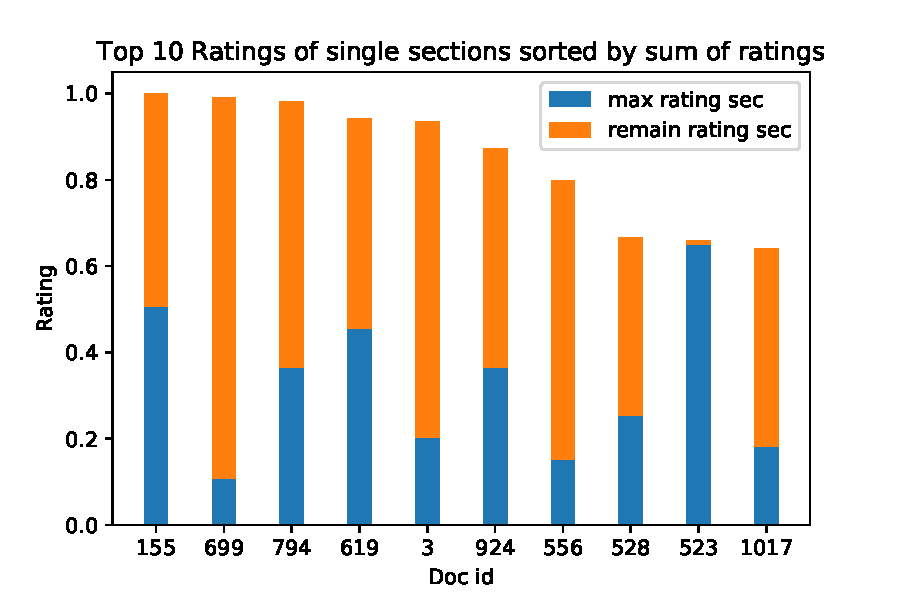
\includegraphics[width=.8\textwidth]{2000_only_sec_sorted_by_sum} 
	\end{figure}
}

\frame{
	\frametitle{Query:"game", adding the rank for the whole page}
	
	\begin{figure}
		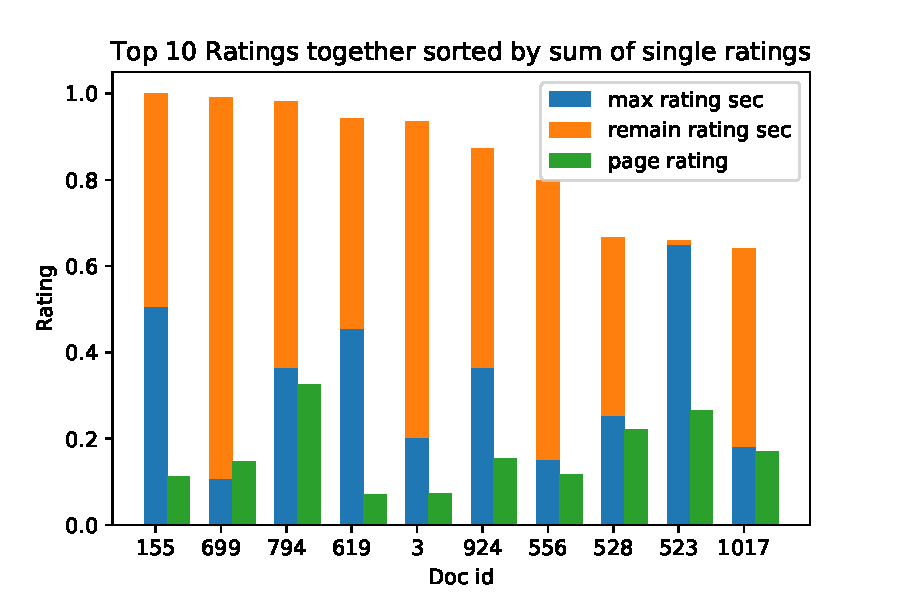
\includegraphics[width=.8\textwidth]{2000_together_sroted_by_sum} 
	\end{figure}
}

\frame{
	\frametitle{Query:"game", ordered by max section rating}
	
	\begin{figure}
		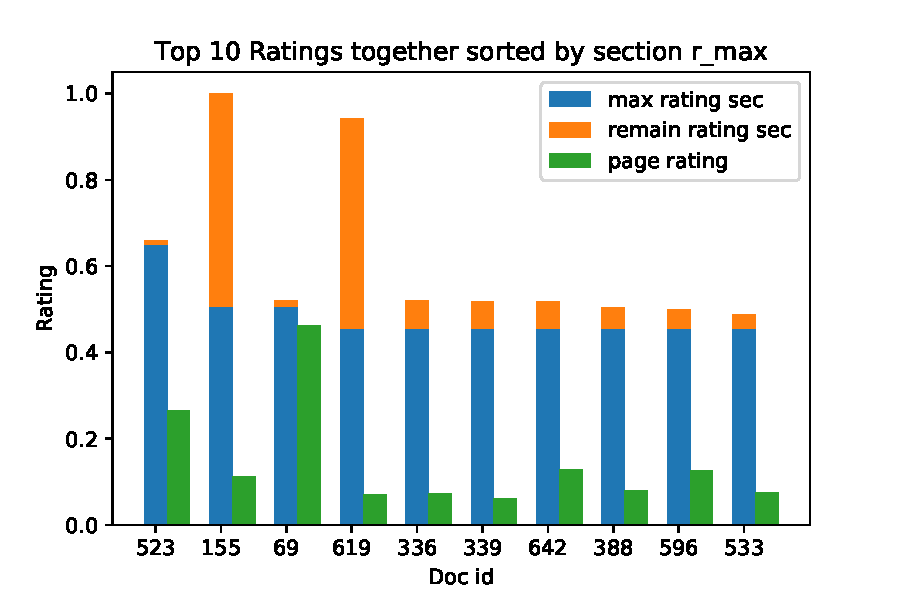
\includegraphics[width=.8\textwidth]{ordered_by_rmax_together} 
	\end{figure}
}

\frame{
	\frametitle{Query:"game AND team AND ball", ordered by max section rating}
	
	\begin{figure}
		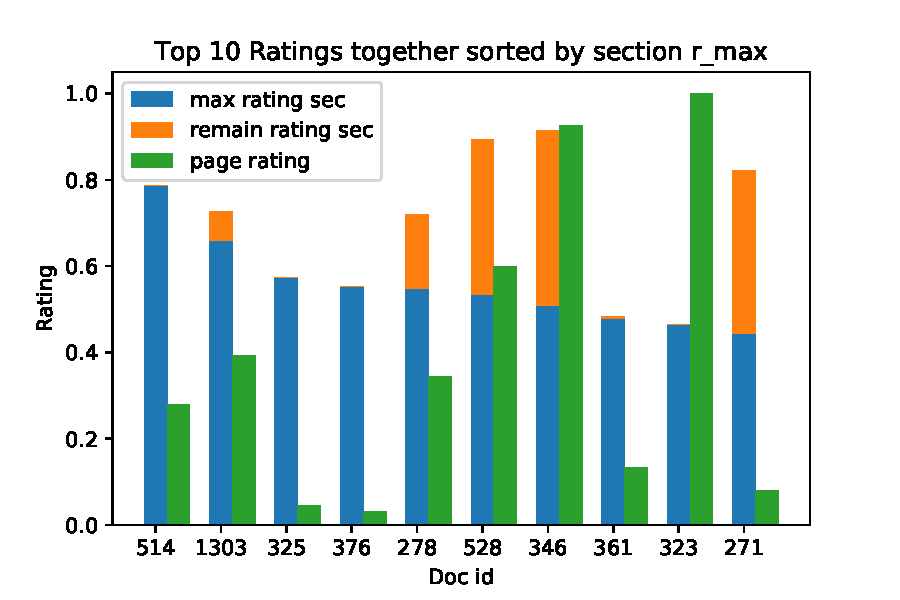
\includegraphics[width=.8\textwidth]{tripel_ordered_by_rmax_together} 
	\end{figure}
}



%========================================
%========================================

\section[Conclusion]{Conclusion}

\subsection{Conclusion}

\frame{
	\frametitle{Conclusion and future work}
	\begin{block}{\centering Conclusion}
		\begin{itemize}
			\item Ratings for sections and page return total different results
			\item Tsvector has a lot of potential
			\item PostgreSQL is easy customizable
		\end{itemize}
	\end{block}

	\begin{block}{\centering Future work}
		\begin{itemize}
			\item Improve the rating algorithm with tf idf information (ts\_stat)
			\item Tests on big datasets
		\end{itemize}
	\end{block}	
}


\frame{\frametitle{Questions}
	%\begin{figure}
	%
\includegraphics[width=.8\textwidth]{questions} 
	%\end{figure}
	\vspace*{2.3cm}\begin{center}\begin{LARGE}\textbf{Questions}\end{LARGE}\end{center}
	\vspace*{2cm}
}

\end{document}
